\documentclass{article}
\usepackage{gvv-book}
\usepackage{gvv}
\usepackage{amsmath}
\usepackage{amsfonts}
\usepackage{tikz}
\usepackage{setspace}
\usepackage{gensymb}
\usepackage[cmex10]{amsmath}
\usepackage{amsthm}
\usepackage{mathrsfs}
\usepackage{txfonts}
\usepackage{stfloats}
\usepackage{bm}
\usepackage{cite}
\usepackage{cases}
\usepackage{subfig}
\usepackage{longtable}
\usepackage{multirow}
\usepackage{enumitem}
\usepackage{mathtools}
\usepackage{tikz}
\usepackage{circuitikz}
\usepackage{verbatim}
\usepackage[breaklinks=true]{hyperref}
\usepackage{tkz-euclide}
\usepackage{listings}
\usepackage{color}    
\usepackage{array}    
\usepackage{longtable}
\usepackage{calc}     
\usepackage{multirow} 
\usepackage{hhline}   
\usepackage{ifthen}   
\usepackage{lscape}     
\usepackage{chngcntr}
\usepackage{graphicx}
\usepackage{float}
\usepackage{multicol}
\usepackage[a4paper, left = 1.5cm, right = 1.5cm]{geometry}

\begin{document}

\begin{center}
\large
    \textbf{Samyak Gondane-AI25BTECH11029}
\end{center}
\date{}

\section*{Question}
If the latus rectum of an ellipse is equal to half of minor axis, then find its eccentric

\section*{Solution}





\subsection*{Parametric Vector Form of Ellipse}

An ellipse centered at the origin is defined by the vector function:


\begin{align}
\vec{r}(\theta) =
\myvec{
x(\theta) \\
y(\theta)
}
=
\myvec{
a \cos \theta \\
b \sin \theta
}
\quad \text{where } \theta \in [0, 2\pi]
\end{align}



Here, $a$ and $b$ are the semi-major and semi-minor axes respectively.

\subsection*{Focus and Latus Rectum}

The focus of the ellipse lies at:


\begin{align}
\vec{F} = 
\myvec{
ae \\
0
}
\quad \text{where } e = \text{eccentricity}
\end{align}



The latus rectum $L$ is the chord perpendicular to the major axis passing through the focus:


\begin{align}
L = \frac{2b^2}{a}
\end{align}



\subsection*{Given Condition}

We are given:


\begin{align}
L = \frac{1}{2} \cdot 2b = b
\quad \Rightarrow \quad \frac{2b^2}{a} = b
\quad \Rightarrow \quad 2b = a
\end{align}



Thus:


\begin{align}
a = 2b
\end{align}



\subsection*{Eccentricity via Vector Displacement}

Eccentricity is defined as:


\begin{align}
e = \frac{c}{a}
\quad \text{where } c = \text{distance from center to focus} = \sqrt{a^2 - b^2}
\end{align}



Substitute $a = 2b$:


\begin{align}
c = \sqrt{(2b)^2 - b^2} = \sqrt{4b^2 - b^2} = \sqrt{3b^2} = b\sqrt{3}
\end{align}





\begin{align}
e = \frac{b\sqrt{3}}{2b} = \frac{\sqrt{3}}{2}
\end{align}



\subsection*{Final Answer}



\begin{align}
\boxed{e = \frac{\sqrt{3}}{2}}
\end{align}



\begin{figure}[H]
    \centering
    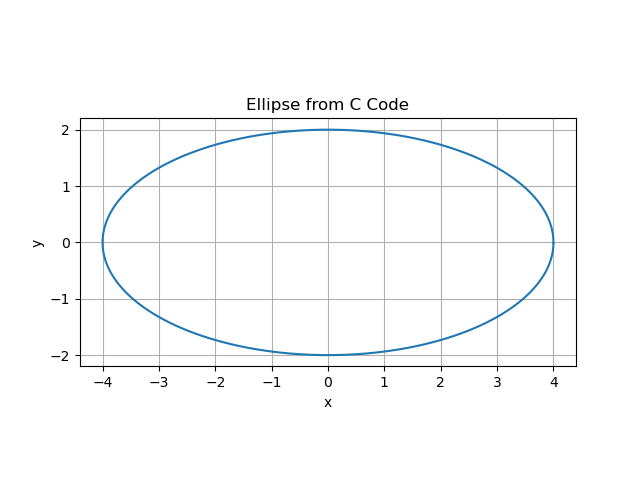
\includegraphics[width=0.7\linewidth]{./figs/Figure_1.png}
    \caption{}
    \label{fig:fig1}
\end{figure}

\end{document}